% !TEX root = ../report.tex

\chapter{Design}

\minitoc
This chapter describes the architecture and components in the architecture, how they were designed, and how they fulfill the requirements of the project.

\clearpage

\section{Architecture}
The architecture of the project is based on The 4+1 View Model of Software Architecture \cite{Kruchten}. The views are used to reflect the structural aspects, temporal aspects, technological development aspects and physical aspects of the project.

The architecture uses a custom simplified version of the 4+1 notation that better fits the descriptive needs for the project.


\subsection{Logical View}
The logical view describes the components of the architecture and how they relate to one another in terms of containment, inheritance and usage. The logical view can be found in figure~\ref{figure:logical-view} and the notation for the logical view in figure~\ref{figure:logical-view-notation}

\begin{figure}[H]
\centerline{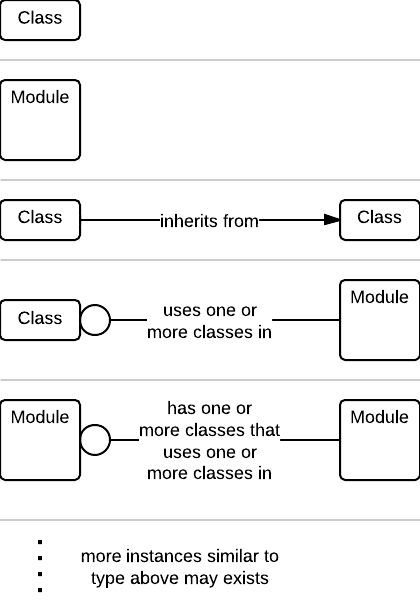
\includegraphics[width=2.5in]{image/architecture-logical-view-notation.png}}
\caption[Notation for the logical view]{Notation for the logical view.}
\label{figure:logical-view-notation}
\end{figure}

\begin{center}
\begin{figure}[H]
\centerline{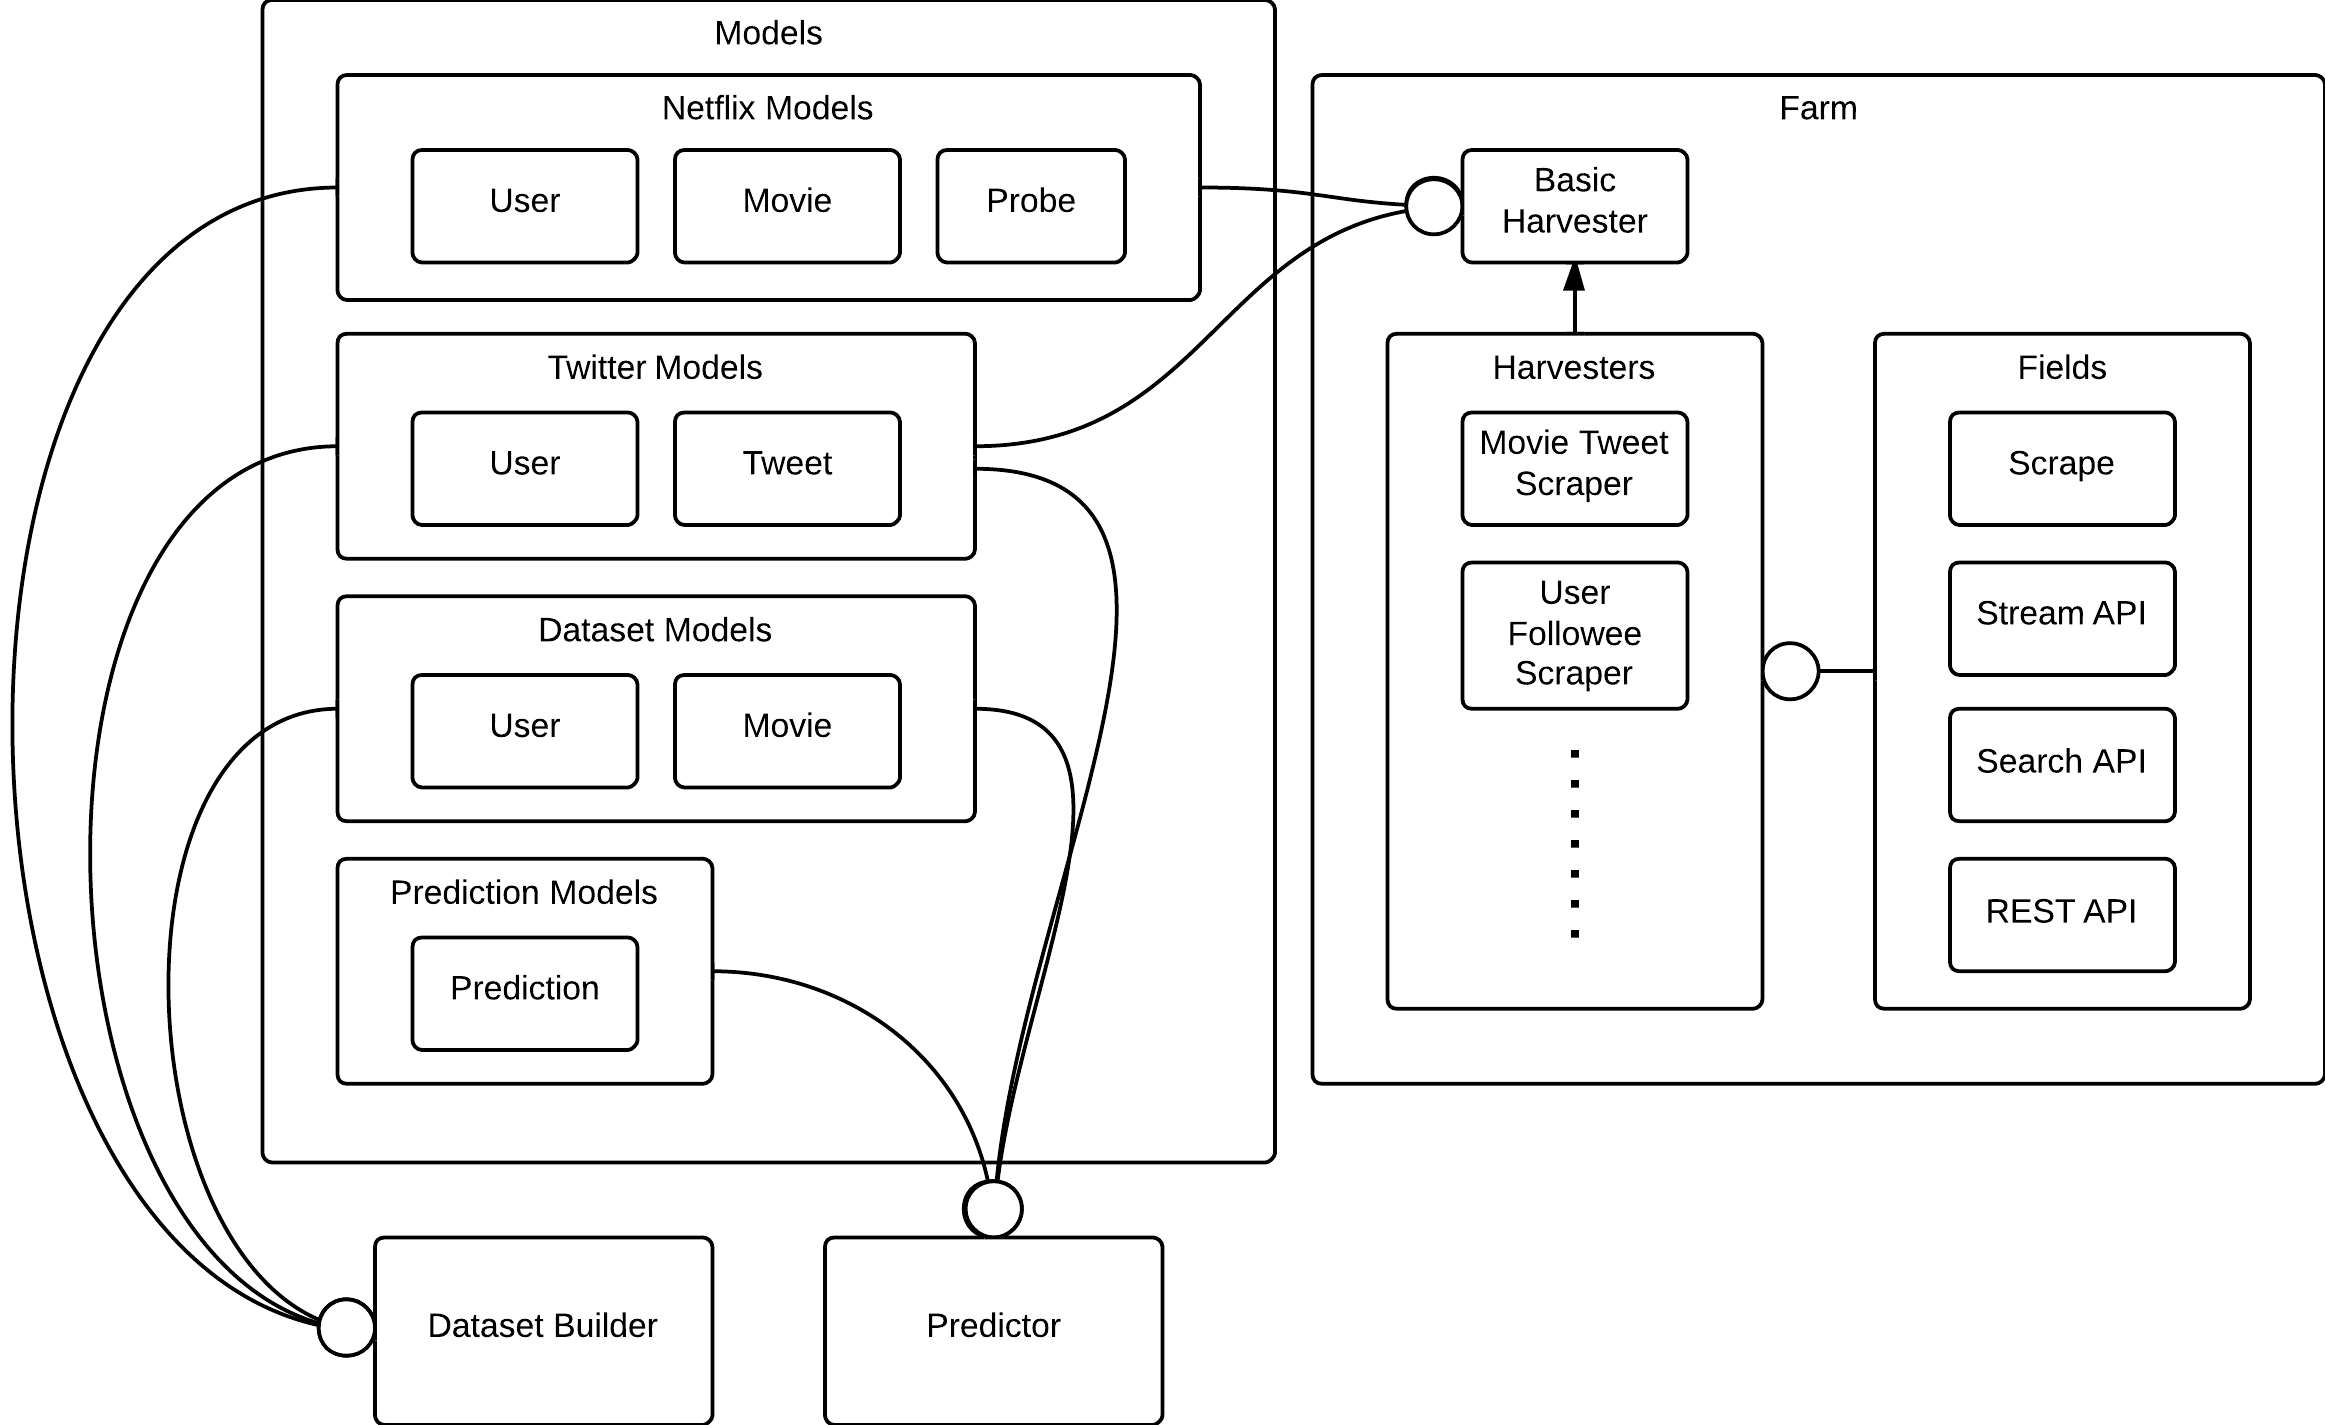
\includegraphics[width=7in]{image/architecture-logical-view.png}}
\caption[Logical view]{Logical view of the project. See figure~\ref{figure:logical-view-notation} for notation.}
\label{figure:logical-view}
\end{figure}
\end{center}

\subsubsection{Models}
Models is the module responsible for holding the different data models that are used in the project. It is found in the upper left part of the logical view in figure~\ref{figure:logical-view}. All classes in this module are mapped to and reflect the database.

The Netflix Models model the Netflix Prize dataset. Each user has a list of movie ratings and each movie has a list of user ratings. The probe is a list of movies with empty user ratings that need to be predicted.

The Twitter Models reflect the data harvested from Twitter. The schema of these models are variable as it depends on what type of data is harvested. A tweet typically contains a text and refers to a user. A user typically has a name and a user ID and may refer to tweets. As an example, it may also contain a list of followees or followers.

The Dataset Models reflects the Netflix Models after they have been mapped to fused with Twitter Models by the Dataset Builder.

The Prediction Models model what the ratings that the Predictor predicts using the Datast Models and the Probe in Netflix Models.

\subsubsection{Farm}
Farm is the module responsible for accessing and gathering data from Twitter.

The fields access Twitter's data. Most fields implement one of Twitter's existing APIs. There is also a Scrape field for accessing Twitter's web search and scraping the results. It is important to note that Twitter does not allow this without explicit consent. Each field is implemented in such a way that it delivers a subset of the Twitter data types that are outlined in the functional requirements in section~\ref{section:functional-requirements}. The fields combined delivers all the Twitter data types in the requirements. The reason for dividing the access over several fields is that some of the fields are unsuitable for gathering certain Twitter data types.

The harvesters uses the fields to gather and store Twitter data that matches a model that already exists in either the Netflix model or the Twitter model. It is used for finding say tweets for a movie using the scraper field, followees for a user using the rest field or users for a movie using the stream field.

\subsubsection{Dataset Builder}
The dataset builder is responsible for building a dataset that reflects the Netflix dataset using the data gathered from Twitter by the harvesters. This new dataset is stored in dataset model.

\subsubsection{Predictor}
The predictor is responsible for predicting movie ratings for a collection of users. The predictor does this by taking a test set and comparing it to several entries in a dataset. The test set is usually the probe in the Netflix models. The dataset that the test set is compared to, is either the dataset model or the Netflix model. The predictor also gradually calculates RMSE as it is predicting ratings.

\subsection{Process View}
The process view describes the actions that the components of the architecture are engaged in over time, and how their actions relate to other components. See figure~\ref{figure:process-view}

\begin{figure}[H]
\centerline{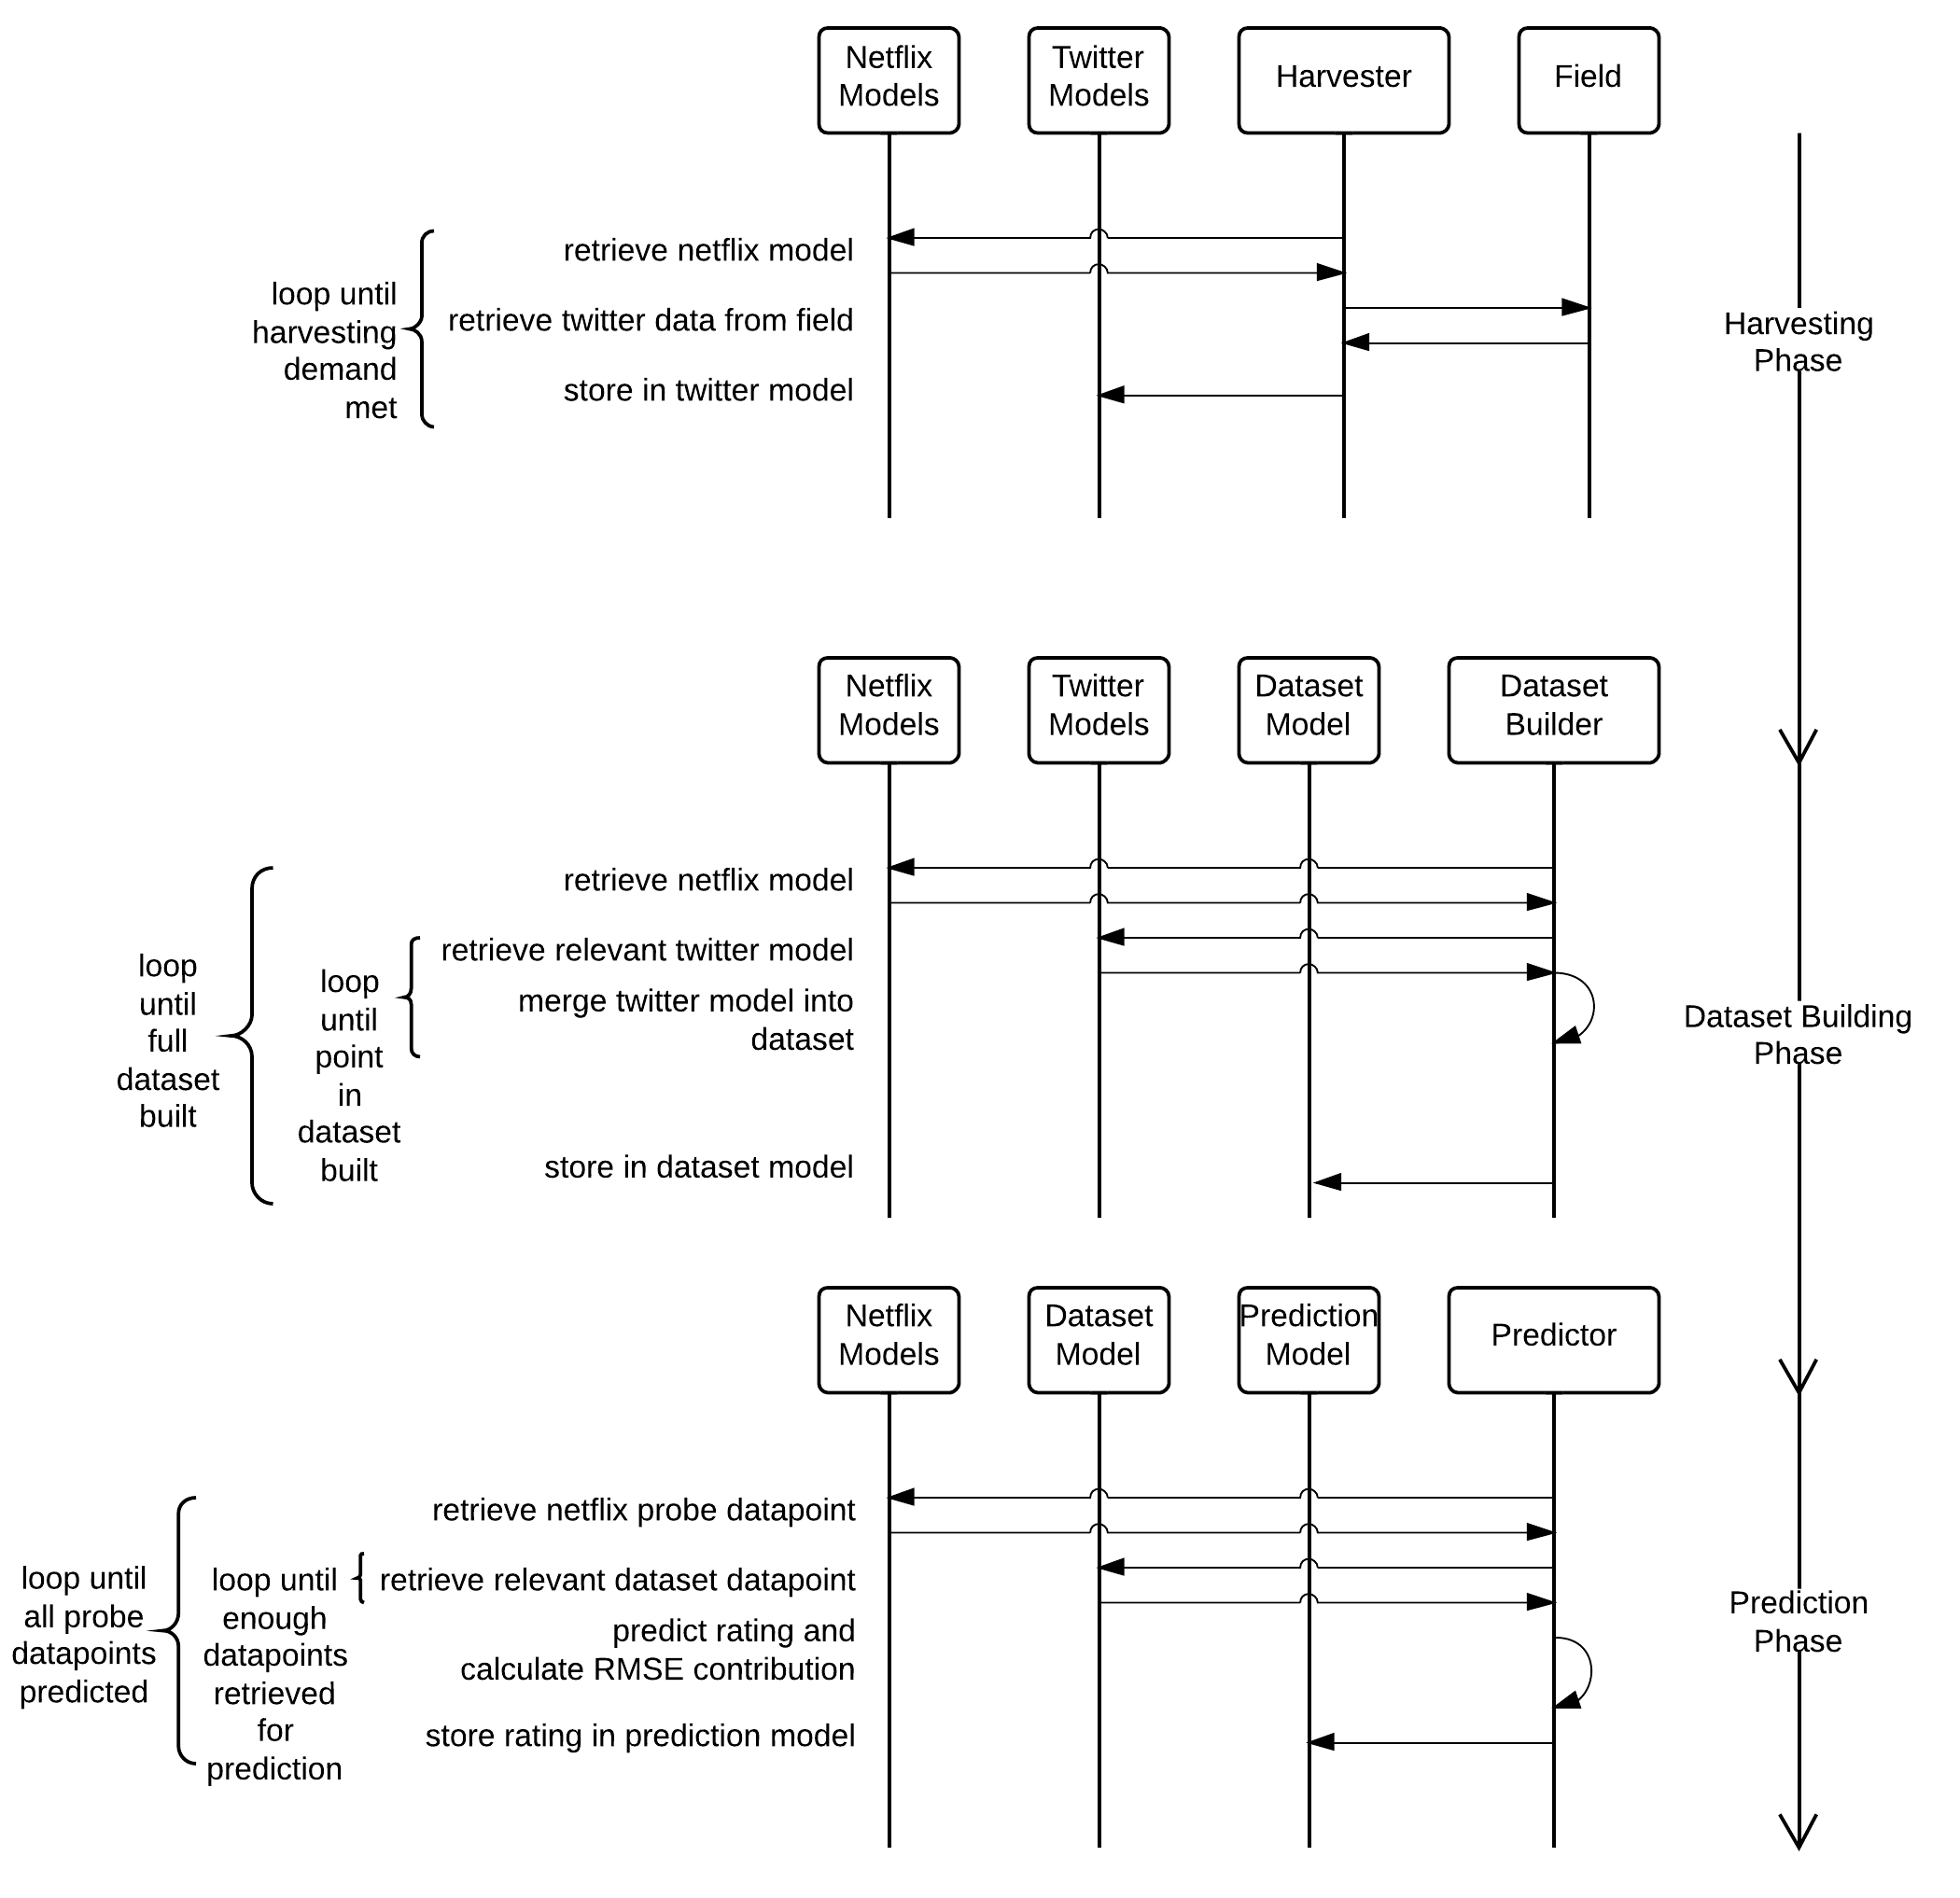
\includegraphics[width=7in]{image/architecture-process-view.png}}
\caption[Process view]{Process view showing the actions taken by various components as time passes and which components they affect. Time is moving downward. An arrow implies that data is sent from one component to another. The data being sent can be a function call, an object or any other type available to the component taking the action.}
\label{figure:process-view}
\end{figure}

\subsubsection{Harvest Phase}
The harvest phase is responsible for gathering data from Twitter. First, the harvester retrieves an initial model from either Netflix models or Twitter models. Then, it uses one or more fields to harvest data from Twitter that is related to the initial model. This can be tweets containing the movie title in the tweet.text, tweet.users for these tweets, users.each.followees and so forth, as outlined in the functional requirements related to harvesting in section~\ref{section:functional-requirements}. At last, the harvested data is stored as Twitter models.

\subsubsection{Dataset Building Phase}
The dataset building phase is responsible for building a dataset using the data gathered from Twitter in the harvest phase. First, the dataset builder retrieves a Netflix model, which is likely to be a movie. Then, it retrieves Twitter models that are relevant for the Netflix model and consolidates them into a set of data points that expresses this Netflix model. At last, the data points are stored along with the Netflix model it expresses in the dataset model. In this way, the functional requirement in section~\ref{section:functional-requirements} for supplementing the Netflix Prize dataset with data from Twitter is fulfilled.


\subsubsection{Prediction Phase}\label{subsubsec:predict-phase}
The prediction phase is responsible for using the dataset model to predict the ratings of the probe in the Netflix model and calculate the RMSE. First, the predictor retrieves a data points from the probe. Then, it gathers the relevant data points it needs from the dataset model in order to make a prediction. After this step, the rating has been predicted and the contribution to the RMSE score is calculated. The RMSE contribution is summed in the predictor and kept until all ratings have been predicted. At last, the predicted rating is stored in the prediction model. When all ratings have been predicted and all the RMSE contributions have been added to the prediction model, the RMSE can be calculated and stored. Thus, the functional requirements in section~\ref{section:functional-requirements} related to giving and testing predictions are fulfilled.

\subsection{Development View}
The development view describes how the various technologies and implementations are dependent on one another. A layered approach is used to depict this in figure~\ref{figure:development-view}. It shows how the commercial off-the-shelf software (COTS) is dependent on the underlying language they are built in. Also, it shows how the modules implemented in the project are dependent on the various COTS.

\begin{figure}[H]
    \centerline{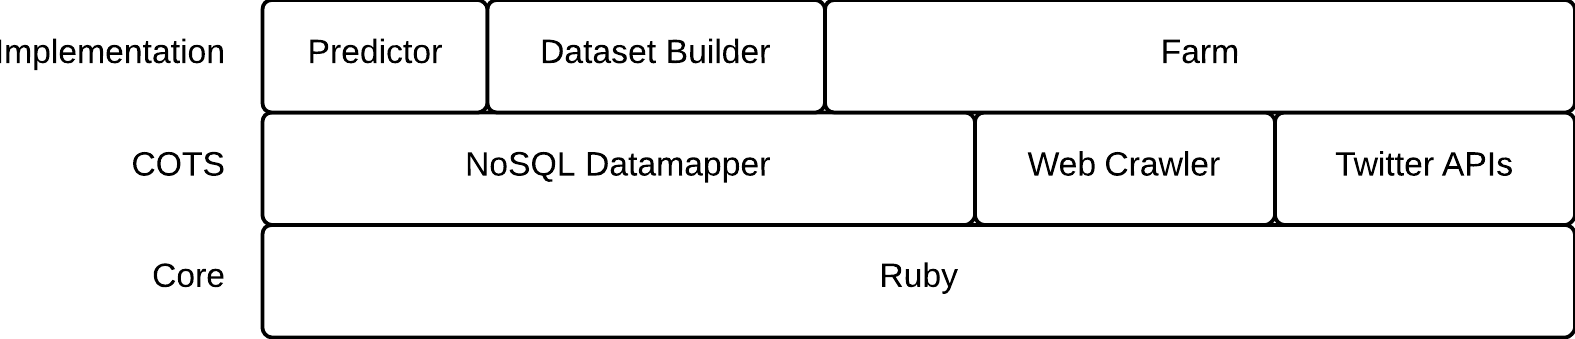
\includegraphics[width=4.5in]{image/architecture-development-view.png}}
    \caption[Development view]{Development view showing the technology stack. Each technology block is dependent on the technology block(s) below it.}
    \label{figure:development-view}
\end{figure}

\subsection{Physical View}
The physical view describes the mapping(s) of the software onto hardware, as seen in figure~\ref{figure:physical-view}. The NoSQL database communicate with the Twilm implementation. These are both stored on a single computer. This computer has Internet access. The Twilm implementation uses the Internet access to reach Twitter.

The NoSQL database can also be decoupled from the computer running Twilm and set up on several computers with replication, as shown in figure~\ref{figure:distr-phys-view}. This fulfills the system storage replication requirement in the non functional requirements in section~\ref{section:non-functional-requirements}.

\begin{figure}[H]
\centerline{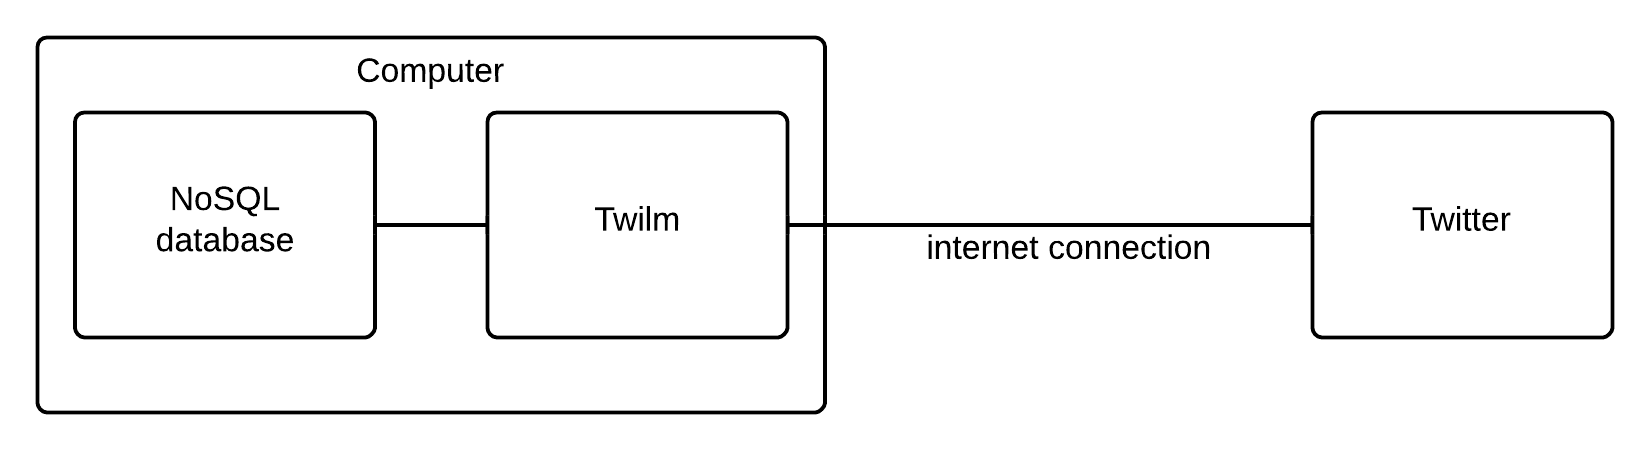
\includegraphics[width=4.5in]{image/architecture-physical-view.png}}
\caption[Physical view]{Physical view showing the components of the system mapped onto hardware. Only a single computer with Internet access to Twitter runs the entire system.}
\label{figure:physical-view}
\end{figure}

\begin{figure}[H]
\centerline{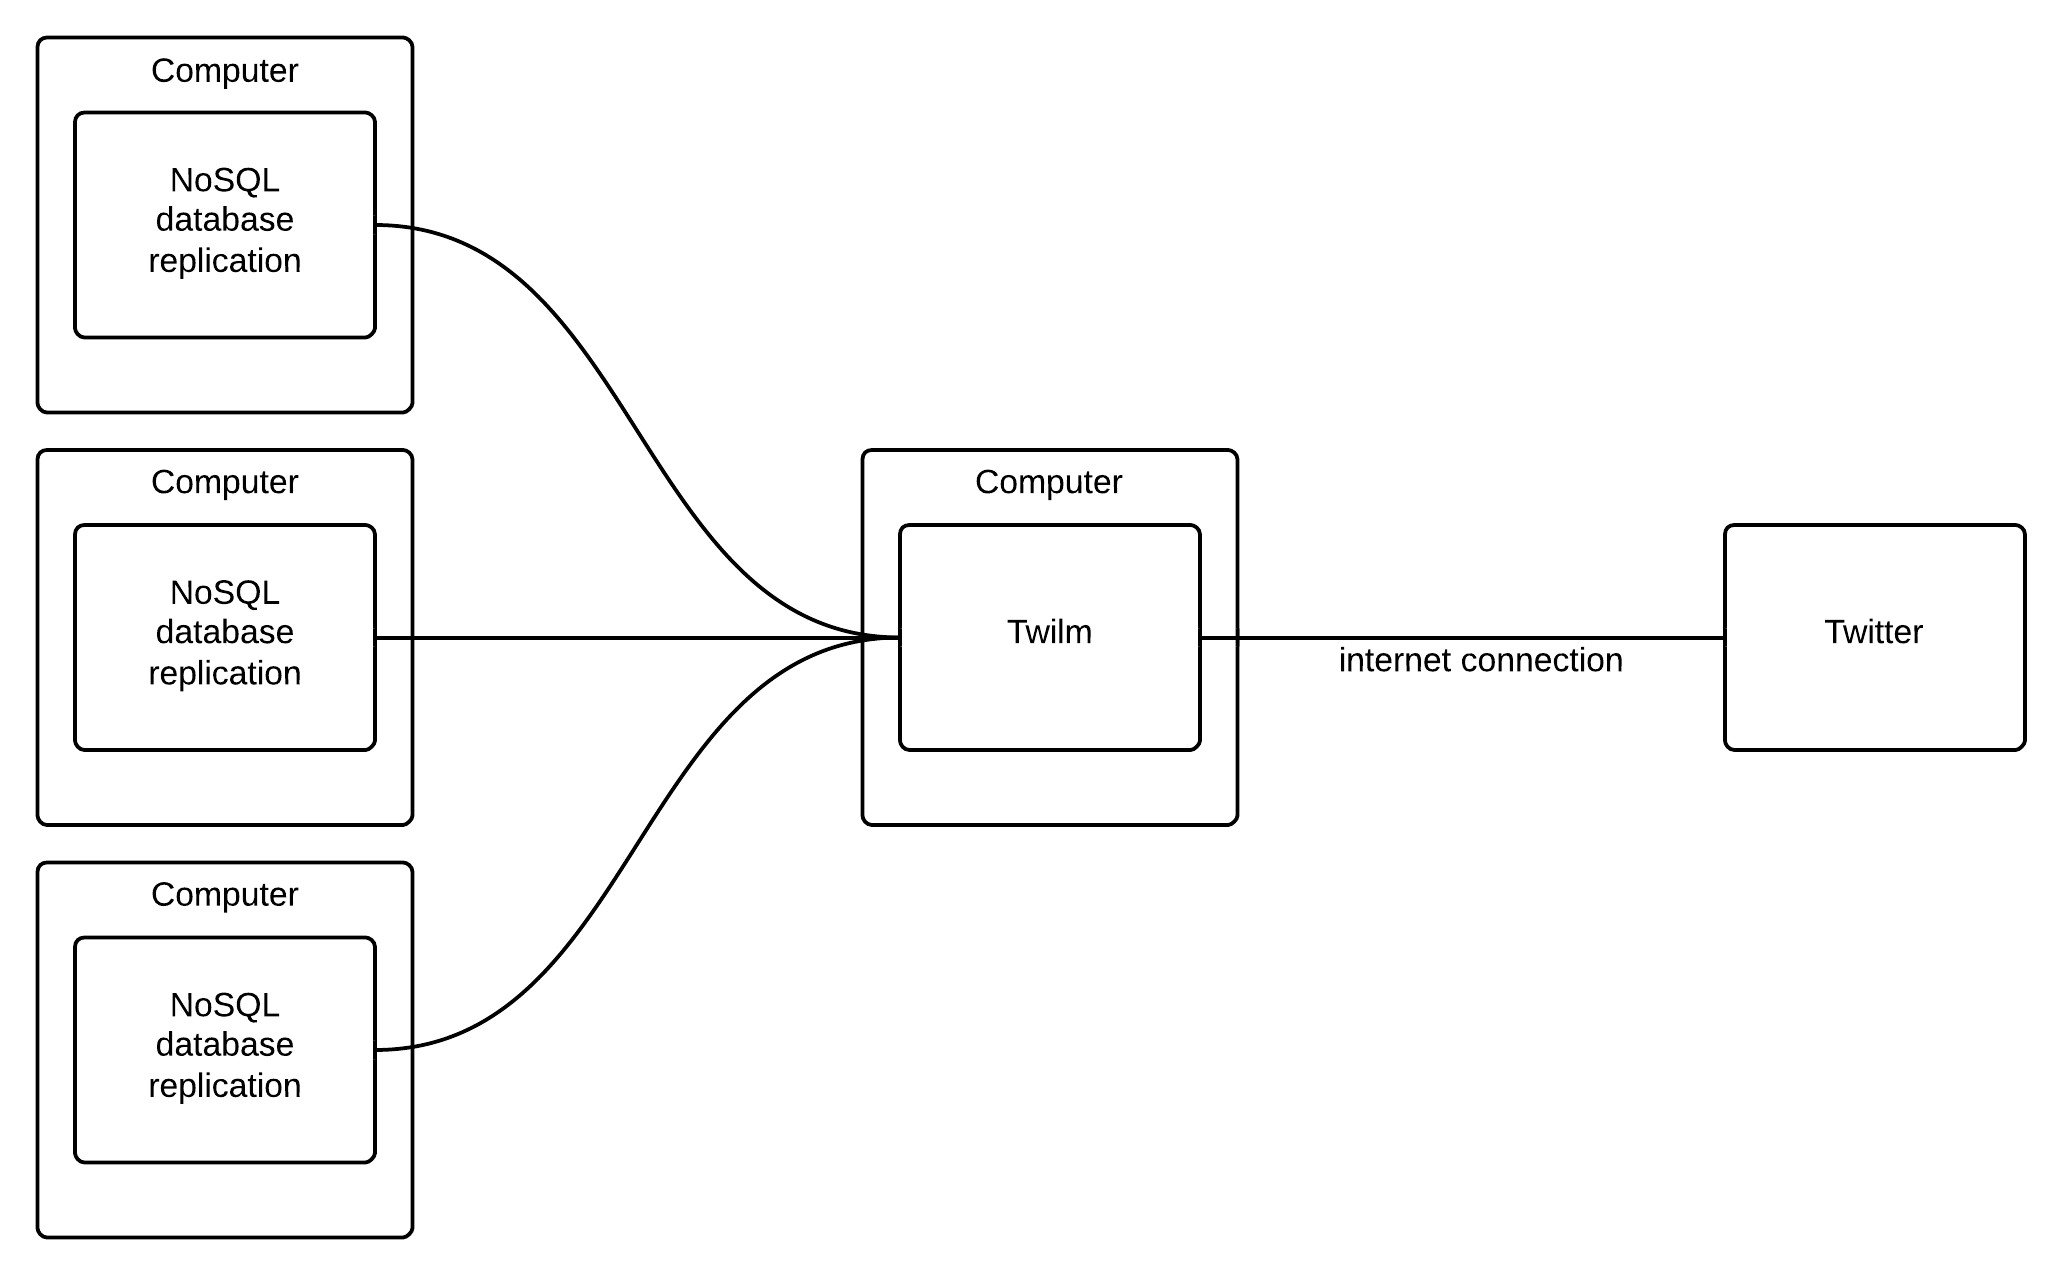
\includegraphics[width=4.5in]{image/architecture-physical-view-distributed.png}}
\caption[Distributed physical view]{Distributed physical view showing the components of the system mapped onto hardware using database replication.}
\label{figure:distr-phys-view}
\end{figure}

\section{Algorithm Design}
\subsection{Dataset Building}\label{algorithm-design:dataset-building}
The dataset building algorithm retrieves and iterates over a list of Netflix users in a test set. This test set is normally the probe in the Netflix Prize dataset. It then consolidates Twitter data with Netflix Prize data by building a dataset for the user based on Twitter data points related to the movies the user has rated. An illustration of this process and its beginning and resulting data structures can be seen in figure~\ref{figure:dataset-building-algorithm}

\begin{figure}[H]
    \centerline{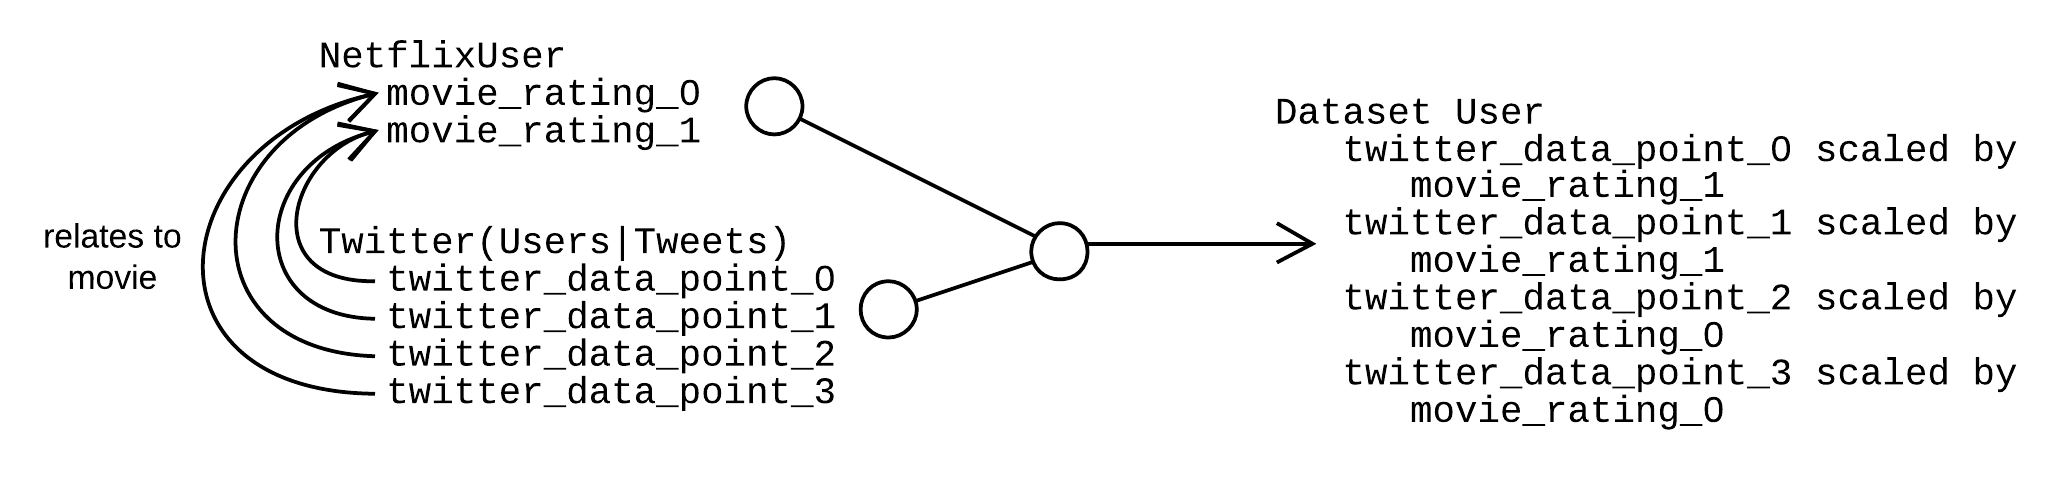
\includegraphics[width=6in]{image/design-algorithm-dataset-building.png}}
    \caption[Database building algorithm]{Illustration of the dataset building algorithm. The algorithm retrieves data about a Netflix user and consolidates it with the Twitter data points related to the movies the user has rated.}
    \label{figure:dataset-building-algorithm}
\end{figure}


\subsubsection{Retrieval}
    Each Netflix user that is not present in the test set is retrieved and iterated over.
    For each of the movies that these users have rated, the corresponding movie in the dataset that is being built containing the Twitter data points that are relevant to the movie is retrieved.
    If the dataset does not yet contain this movie, the relevant Twitter data points are retrieved from the Twitter model and added to the dataset movie.

\subsubsection{Consolidating}
	Once Twitter data points that are related to a movie a user has rated have been retrieved, these data points must be consolidated with the user's data points. The user data points is a hash of Twitter data points that point to a number indicating whether or not the user is positively or negatively interested in this Twitter data point. Each Twitter data point related to the movie the user has rated is added to this hash and scaled by whether or not the user liked it. After Twitter data points have been added to the user data points for all movies the user has rated, they are normalized to a scale of [0, 1] for each user. The user is now expressed in the dataset entirely by Twitter data points rated from 0 to 1.

\subsection{Prediction}\label{algorithm-design:prediction}
As mentioned in \ref{subsubsec:predict-phase} the system must produce a prediction on the dataset. As concluded in the preliminary study the most suitable algorithms to produce these predictions for this kind of dataset has proven to be a k-nearest neighbors (k-NN) approach. This is because it will allow a low response time, but yet has produced good prediction results on the Netflix Prize dataset~\ref{subsec:sim-sys-conc}.

There are many approaches to gather and select neighbors to calculate predictions with, but the approach which seems most promising is the probabilistic neighborhood selection~\cite{probcobfilter}, and is the approach to be taken.

The prediction algorithm design is split into 3 parts. The last part depends on if the prediction was issued because a user rated a movie, or a movie prediction rating was requested.

\begin{description}
    \item[First - Retrieval part] \hfill \\
    The system will retrieve the data points closest to the point to predict. These points are retrieved with a k-NN algorithm, which utilizes a probabilistic selection when selecting neighbors.

    \item[Second - Evaluation part] \hfill \\
    The neighbors returned are evaluated. A prediction based on the data points is produced, and a confidence measure on this prediction is produced.

    \item[Third - Learning part] \hfill \\
    If a user rated a movie, the actual rating is compared with the predicted rating, and the data points are weighted regarding of the accuracy of the rating.
\end{description}

\begin{figure}[H]
\centerline{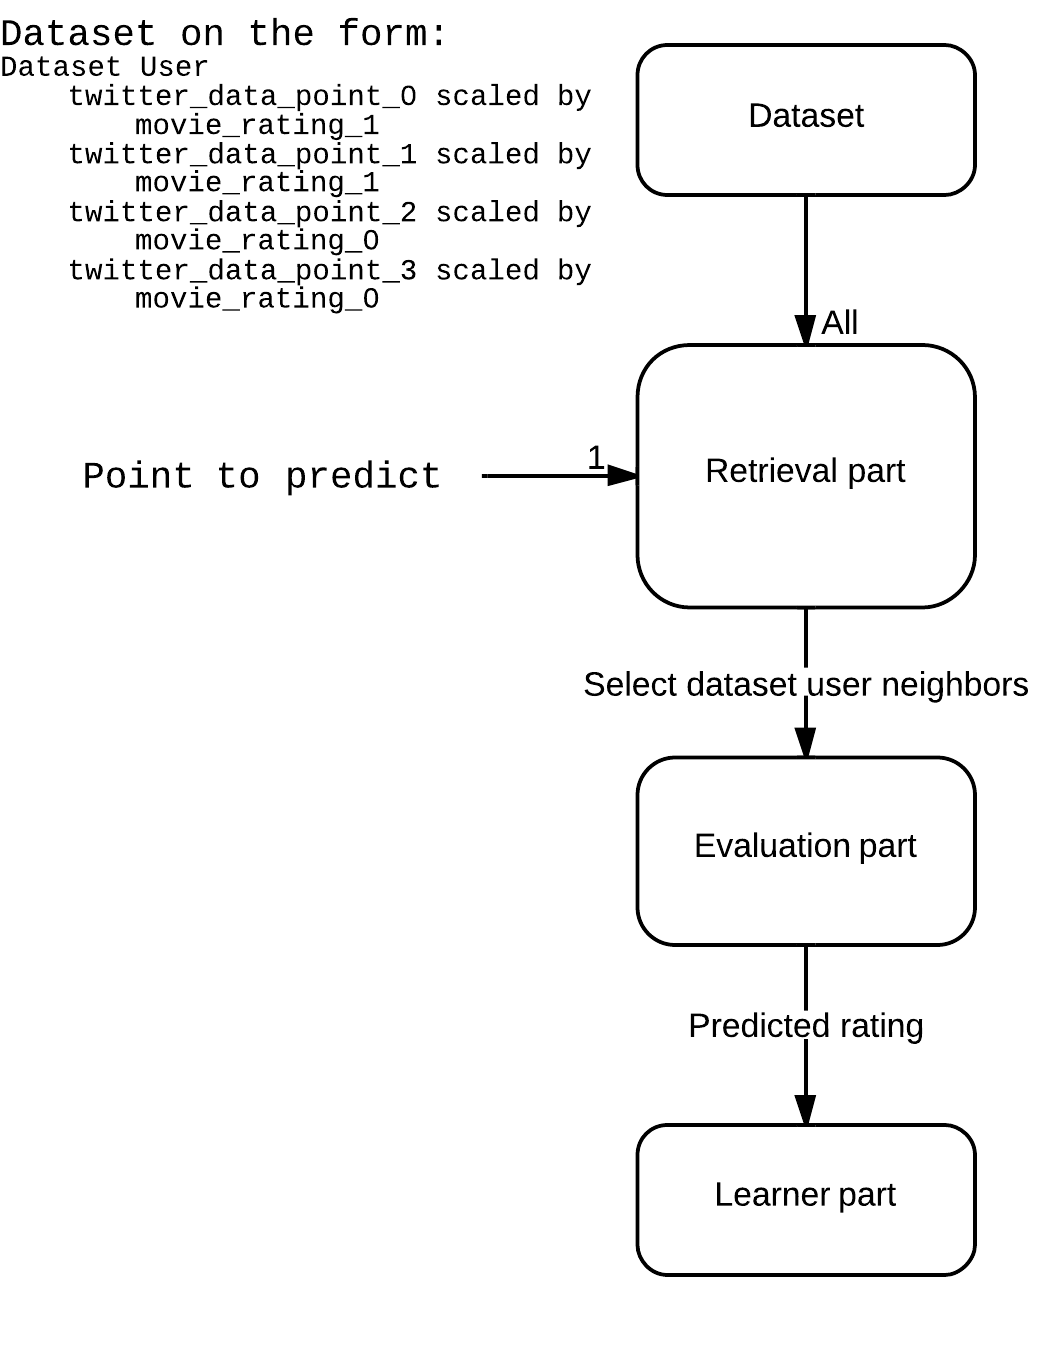
\includegraphics[width=3.5in]{image/pred-alg.png}}
\caption[Prediction algorithm]{The prediction algorithm design and the parts it is separated into. The dataset consist of users on the form described in the top. With the given point the neighbors are selected from the dataset. This is then sent to the evaluation part. Here a prediction is produced.}
\label{figure:pred-alg}
\end{figure}
